\documentclass[a4paper,fontsize=12pt,toc=bib,halfparskip]{scrartcl}

\usepackage[utf8]{inputenc} % utf8 input encoding
\usepackage{lmodern} % font
\usepackage[T1]{fontenc} % 8-Bit output encoding
\usepackage[ngerman]{babel} % This is a (new)german document so we want to have german labels as well
\usepackage[dvipsnames]{xcolor} % refer to some colors by name
\usepackage{graphicx} % able to load more graphic formats
\usepackage[pdfborder={0 0 0},colorlinks,urlcolor=NavyBlue,linkcolor=NavyBlue,citecolor=NavyBlue]{hyperref} % make clickable hyper links in documents
\usepackage[headsepline,plainheadsepline]{scrpage2} % for header and footer layout
\usepackage{nag} % for not using forbidden things referenced in l2tabu
\usepackage{blindtext} % for inserting blind text
\usepackage[backend=biber, style=numeric]{biblatex} % for references
\usepackage{xspace} % inserts missing space at the end of custom commands
\usepackage{amsmath} % for cool math stuff
\usepackage{microtype} % for better kerning
\usepackage{array}
\usepackage{subcaption}
\usepackage[german]{algorithm2e}
\usepackage{amsmath} 
\usepackage{amssymb}
\usepackage{svg}
\addbibresource{Literatur.bib} % database for references
\graphicspath{{./images/}} % sets the default path for images

% header and footer settings
\pagestyle{scrheadings}
\clearscrheadfoot
\newcommand{\veranstaltung}{Schematische 2D Visualisierung von RNA-Protein Interaktionen\xspace}
\lohead{\veranstaltung}
\rohead{\headmark}
\setfootsepline{0.1pt}
\ofoot{\textsf{\thepage/\getpagerefnumber{LastPageBeforeRefs}}}

% title page
\renewcommand*{\titlepagestyle}{empty}
\addto\captionsngerman{\def\figurename{Abb.}}
\subject{Masterarbeit}
\title{Schematische 2D Visualisierung von RNA-Protein Interaktionen\xspace}
\newcommand{\matrikelnummer}{2878372\xspace}
\author{Niklas Teichmann}
\date{\today}
\newcommand{\kurz}{Die Visualisierung von Tensorfeldern ist trotz vielen Jahrzehnten aktiver Forschung noch immer ein aktives Thema. Komplexe Strukturen innerhalb von Tensorfeldern stellen hohe Anforderungen an Visualisierungssoftware, um die Interpretation durch Benutzer zu erleichtern. Innerhalb dieser Arbeit wurde eine Erweiterung f\"ur die Visualisierungssoftware `FAnToM' entwickelt, die Techniken aus dem Direct Volume Rendering und dem Continuous Scatterplotting verwendet, um Invarianten von symmetrischen Tensoren 2. Grades und ihre Verteilung innerhalb eines Datensatzes darzustellen. Dabei wurde besonderer Wert auf Interaktivit\"at gelegt, um Nutzern die explorative Analyse der Daten zu erm\"oglichen.}

% renders abstract along with declaration at titlepage with \publishers workaroung
\publishers{%
    \normalfont\normalsize%
    \vspace{2cm}
    \parbox{\linewidth}{\textbf{Zusammenfassung}:~\kurz}\vfill
    \footnotesize
    \parbox{\linewidth}{\textsf{Hiermit erkläre ich, die vorliegende wissenschaftliche Arbeit selbständig und ohne unzulässige fremde Hilfe
    angefertigt zu haben. Ich habe keine anderen als die angeführten Quellen und Hilfsmittel benutzt und sämtliche Textstellen, die wörtlich oder
    sinngemäß aus veröffentlichten oder unveröffentlichten Schriften entnommen wurden, und alle Angaben, die auf mündlichen Auskünften beruhen, als
    solche kenntlich gemacht. Ebenfalls sind alle von anderen Personen bereitgestellten Materialen oder erbrachten Dienstleistungen als solche
    gekennzeichnet.}}\vspace{0.4cm}
    \parbox{\linewidth}{\textsf{Leipzig, d. \underline{\hspace{2cm}} \hfill \underline{\hspace{4cm}}\newline Ort, Datum \hspace{3.0cm} Matrikelnummer: \matrikelnummer \hfill Unterschrift}}
}

\begin{document}
\maketitle\clearpage
\thispagestyle{empty}
\tableofcontents\clearpage
\pagenumbering{arabic}

% %%%%%%%%%%%%%%%%%%%%%%%%%%%%%%%%%%%%%%%%%%%%%%%%%%%%%%%%%%%%%%
% START YOUR DOCUMENT HERE
% %%%%%%%%%%%%%%%%%%%%%%%%%%%%%%%%%%%%%%%%%%%%%%%%%%%%%%%%%%%%%%

\section{Einleitung}
Tensorfelder sind eine sowohl in der Forschung als auch in der Praxis h\"aufig vorkommende Art von Datens\"aetzen. Beispiele daf\"ur sind die Diffusions-Tensor-Bildgebung\cite{basser1994mr}, welche die Diffusion von Wasser in Gewebe wie z.B. dem Hirn untersucht, oder Verformungs-\cite[S.~122]{FundamentalsofStructuralMechanics} und Spannungstensoren\cite[S.~154]{FundamentalsofStructuralMechanics} in der Mechanik. Ein h\"aufig gew\"ahlter Ansatz, um die Interpretation von Tensordaten zu erleichtern, ist die Tensorfeldvisualisierung, ein Teilgebiet der wissenschaftlichen Visualisierung, das sich mit der Erzeugung von f\"ur Menschen verst\"andlichen visuellen Repr\"asentationen von Tensorfeldern besch\"aftigt. Auch diese muss sich jedoch den genannten Herausforderungen stellen. Dabei treten jedoch eine Reihe von Problem auf, von denen einige im Folgenden genannt werden\cite{hlawitschka2014top}\cite{fritzsch2016contiuousScatterplot}:

\paragraph{Menge an Daten pro Tensor}
Ein einzelner Tensor kann, abh\"angig von Grad und Dimension, beliebig viele Datenwerte umfassen. Aber selbst ein Tensor 2. Grades und 3. Dimension besteht bereits aus 9 Werten, f\"ur die eine passende Darstellung gefunden werden muss.

\paragraph{Menge an Daten pro Datensatz}
H\"aufig enthalten Datens\"atze Tausende oder Millionen von Tensoren, was gut skalierende Werzeuge zur Analyse notwendig macht. Zudem bestehen relevante Merkmale der Datens\"atze oft nur aus wenigen Datenpunkten, weshalb effektives Filtern wichtig wird.

\paragraph{Fehlende Intuition}
Tensoren beschreiben im Allgemeinen lineare Abh\"angigkeiten zwischen Skalaren, Vektoren und anderen Tensoren. W\"ahrend bei niedrigen R\"angen (Skalare/Vektoren) noch intuitive Interpretation existieren (Zahlenwert/Punkt im dreidimensionalen Raum), f\"allt es Menschen erheblich schwieriger, Matrizen oder Tensoren h\"oheren Grades zu interpretieren. Die Repr\"asentation eines Tensors muss daher sehr gut durchdacht sein, und relevante Eigenschaften interpretierbar darstellen.

\paragraph{Dom\"anenspezifische Informationen}
Abh\"angig von der jeweiligen Dom\"ane k\"onnen unterschiedliche Informationen \"uber die vorliegenden Tensoren von Interesse sein.  Zum Beispiel kann isotropen oder degenerierten Punkten (Punkte, in denen die Eigenvektoren nicht eindeutig definiert sind) in manchen Anwendungsf\"allen besondere Bedeutung zugemessen werden, w\"ahrend sie in anderen Kontexten nur Punkte hoher Symmetrie ohne besonere Bedeutung sind \cite[S.~4]{hlawitschka2014top}. Eine Anwendung zu entwickeln, die \"uber Dom\"anen hinweg verwendbar ist, ist daher schwer.


Im Zuge der vorliegenden Arbeit wurde ein neues Verfahren zur Visualisierung von symmetrischen Tensoren 2. Grades im dreidimensionalen Raum entwickelt und als Erweiterung der Visualisierungssoftware `FAnToM' implementiert. Im Speziellen wurden Invariantenfelder aus den der Matrixdarstellungen der Tensoren berechnet und mithilfe von Techniken aus dem Continuous Scatterplotting und dem Direct Volume Rendering dargestellt. Durch Mausinteraktionen ist es m\"oglich, Bereiche von Invarianten auszuw\"ahlen und im urspr\"unglichen Feld darzustellen. Das Ziel der Anwendung ist es, Kontinuumsmechanische Untersuchungen von Materialien und Werkst\"ucken zu erleichtern.

Der Rest dieser Arbeit ist wie folgt gegliedert: Zun\"achst werden im Kapitel \hyperref[sec:Verwandte]{2 Verwandte Arbeiten} bekannte Verfahren zur Tensorfeldvisualisierung mit Vor- und Nachteilen erl\"autert. Danach werden im Kapitel \hyperref[sec:Grundlagen]{3 Grundlagen} Definitionen und Grundlagen aus der Mathematik und Kontinuumsmechanik vorgestellt, die in dieser Arbeit verwendet wurden. Als n\"achstes werden in \hyperref[sec:Technologien]{4 Verwendetete Verfahren und Technologien} Programmschnittstellen und Visualisierungstechniken erl\"autert, die innerhalb dieser Arbeit verwendet wurden. Insbesondere wird dort auch auf FAnToM als Softwaregrundlage eingegangen. Kapitel \hyperref[sec:Umsetzung]{5 Umsetzung} beschreibt die konkrete Umsetzung der FAnToM-Erweiterung mit allen implementierten Funktionen. Nachfolgend werden in Kapitel \hyperref[sec:Ergebnisse]{6 Ergebnisse} wird die entwickelte Erweiterung exemplarisch auf einige Datens\"atze angewendet, und die Ergebnisse diskutiert. Zum Abschluss werden in Kapitel \hyperref[sec:Ausblick]{7 Ausblick} im Verlauf dieser Arbeit neu aufgetretene Problemstellungen sowie weitere Verbesserungsm\"oglichkeiten er\"ortert.
 
\section{Verwandte Arbeiten}
\label{sec:Verwandte}
Es existiert bereits eine gro{\ss}e Anzahl von Verfahren, die Visualisierungen von Tensorfeldern erzeugen. Nachfolgend werden, ohne Anspruch auf Vollst\"andigkeit, einige der wichtigsten genannt und kurz beschrieben.

Eine relative einfache Darstellung eines Vektorfelds besteht darin, die einzelnen Komponenten eines Tensor 2. Grades als Skalarfelder aufzufassen und als Grauwertbild zu zeichnen. Dabei ist der Grauwert an einem Datenpunkt abh\"angig vom Verh\"altniss des Wertes der Komponente des Vektors zu dem h\"ochsten Wert dieser Komponente im Datensatz. Die fr\"uheste gefundene Erw\"ahnung dieses Verfahrens ist in einem Paper von Kindlmann und Weinstein aus dem Jahre 1999 \cite{kindlmann1999hue}, in dem es jedoch als weder neu noch besonders intuitiv beschrieben wird. 

Die wohl verbreiteteste Art von Tensorvisualisierungen sind die glyphenbasierten Verfahren. Diese Verfahren beschr\"ankt sich auf Tensoren zweiten Grades im dreidimensionalen Raum, die als Matrizen dargestellt werden k\"onnen und einen gro{\ss}en Teil der Daten aus Mechanik und Medizin ausmachen. Eine Glyphe ist hierbei ein kleines Bild eines grafischen Primitivs, zum Beispiel eines Ellipsoiden, Kuboiden odern oder Superquadrics\cite{kindlmann2004superquadric}, das einen Tensor darstellt. Die Form der Primitive ist dabei abh\"angig von den Eigenwerten des jeweiligen, als Matrix dargestellten Tensors an dieser Stelle. Indem an jedem Datenpunkt eine solche Glyphe gezeichnet wird, erh\"alt der Benutzer ein Bild von der Verteilung und Struktur der Tensoren im Datensatz. Glyphenbasierte Verfahren sind besonders in der Medizin beliebt, da sie leicht R\"uckschl\"usse auf die Richtung von Nerven- und Muskelfasern zulassen.

Hyperstreamlines\cite{delmarcelle1993visualizing} bilden ein Analogon zu den Stromlinien bei Vektorfeldern. Als Eingabedaten sind nur Felder von reellen, symmetrischen, dreidimensionalen Tensoren 2. Grades mit nichtnegativen Eigenwerten zugelassen, da so sichergestellt wird, dass die Eigenwerte ganzzahlig und gr\"o{\ss}er 0 sind sowie die Eigenvektoren paarweise orthogonal zueinander. Das Verfahren zeichnet ausgehend von festgelegten Punkten Schl\"auche durch das Vektorfeld. Die Mittellinien dieser Schl\"auche entsprechen dabei Stromlinien, deren Richtung vom Eigenvektor mit dem h\"ochsten Eigenwert abh\"angt. Der Durchschnitt durch den Schlauch, orthogonal zur Mitellinie ist stets eine Ellipse, deren Halbachsen den zwei kleineren Eigenwerten entsprechen. Da so aber Informationen \"uber den Wert des gr\"o{\ss}ten Eigenwertes verloren geht, werden einzelne St\"ucken des Schlauchs abh\"angig von diesem Wert eingef\"arbt.

Weiterhin muss die Diplomarbeit von Clemens Fritzsch, `Visuelle Analyse kontinuumsmechanischer Simulationen durch kontinuierliche Streudiagramme'\cite{fritzsch2016contiuousScatterplot}, erw\"ahnt werden, auf der die vorliegende Arbeit direkt aufbaut. Fritzsch verwendet Methoden des Continuous Scatterplottings, um Invarianten von zweidimensionalen, symmetrischen Tensoren 2. Grades darzustellen. Dabei beschr\"ankt er sich jedoch auf zwei der drei Invarianten in jedem Invariantensatz, um einen zweidimensionalen Scatterplot zu erzeugen. Die vorliegende Arbeit erweitert diesen Ansatz auf vollst\"andige Invariantens\"atze indem eine dreidimensionale Darstellung erzeugt wird.

\section{Grundlagen}
\label{sec:Grundlagen}
\subsection{Mathematische Grundlagen}
In diesem Teil der Arbeit werden mathematische Grundlagen zu Tensoren, Feldern und Invarianten erl\"autert. Insbesondere f\"ur die Definition von Tensoren sind Vorkenntnisse n\"otig, die ebenfalls erkl\"art werden. 

Eine erheblicher Teil der verwendeten Formeln und Definitionen stammen aus dem Buch `Introduction to vectors and tensors' von R. M. Bowen und C. C. Wang \cite{bowen2008introduction}.

\subsubsection{Urbild und Bild einer Funktion}
Zu jeder Funktion $f: A \rightarrow B$, die Objekten aus der Menge $A$ Objekte aus $B$ zuordnet, l\"asst sich das Bild einer Menge $A' \subset A$ als

\begin{equation}
	f(A'): \{ b \in B | \exists a \in A' : f(a) = b \}
\end{equation}

und das Urbild einer Menge $B' \subset B$ als

\begin{equation}
	f^{-1}(B'): \{ a \in A | \exists b \in B' : f(a) = b\}
\end{equation}

bestimmen. $f(A)$ wird hierbei die Bildfunktion, $f^{-1}(B)$ die Urbildfunktion genannt. 

\subsubsection{Einschr\"ankung einer Funktion}
Gegeben sei eine Funktion $f: A \rightarrow B$. Dann ist $f|_{A'}: A' \rightarrow B$, die Einschr\"ankung von $f$ auf die Menge $A' \subset A$, definiert als 

\begin{equation}
	f|_{A'}(a) = f(a) \text{ f"ur alle } a \in A'
\end{equation}

und auf allen $a \in A, a \notin A'$ nicht definiert. 

\subsubsection{Volumen einer Teilmenge von $\mathbb{R}^n$}
Das $n$-dimensionale Volumen einer Menge $Vol(A), A \subset \mathbb{R}^n$ wird \"uber das Lebesgue-Stieltjes Ma{\ss} definiert\cite{kusolitsch2014mass}. Intuitiv entspricht es in $\mathbb{R}$ der L\"ange, in $\mathbb{R}^2$ dem Fl\"acheninhalt und in $\mathbb{R}^3$ dem Volumen.

Falls f\"ur eine Menge $A$ gilt $Vol(A)=0$, so bezeichnet man diese als Nullmenge.

\subsubsection{Jacobi Matrix}
Die Jacobi Matrix $J_f$ einer differenzierbaren Abbildung $f: \mathbb{R}^n \rightarrow \mathbb{R}^m$ ist eine $m \times n$ Matrix, deren Komponenten die partiellen ersten Ableitungen von $f$ sind. Formal geschrieben gilt also f\"ur die Koordinaten des Urbilds $x_1, \dots, x_n$ und Abbildungen $f_1, ..., f_n$ der einzelnen Komponenten

\begin{equation}
	J_f(a) := 
	\begin{pmatrix}
		\frac{\partial f_1}{\partial x_1}(a) & \dots & \frac{\partial f_1}{\partial x_n}(a)  \\
		\vdots & \ddots & \vdots \\
		\frac{\partial f_m}{\partial x_1}(a) & \dots & \frac{\partial f_m}{\partial x_n}(a) 
	\end{pmatrix}
\end{equation}

Sie entspricht damit der ersten Ableitung in der mehrdimensionalen Analysis. Die Determinante der Jacobi-Matrix $det(J_f)$ wird auch als Funktionaldeterminante bezeichnet, und beschreibt einige Eigenschaften der Funktion $f$. Die f\"ur diese Arbeit wichtigste Rolle spielt der der absolute Wert $|det(J_f)|$ an einem Punkt $p$, die die Expansion bzw. das Schrumpfen der Funktion in der N\"ahe von $p$ beschreibt. F\"ur eine lineare Funktion $f: \mathbb{R}^n\rightarrow \mathbb{R}^n$, deren Funktionaldeterminante in jedem Punkt $p_n \in \mathbb{R}$ gleich ist, bedeutet das mit dem $n$-dimensionalen euklidischen Abstand $||p_1, p_2||_n$

\begin{equation}
	||f(p_1), f(p_2)||_n = det(J_f)\cdot||p_1, p_2||_n
\end{equation}

Indem man das Lebesgue-Stieltjes Ma{\ss} in $\mathbb{R}^n$ mittels des euklidischen Abstands definiert, lassen sich so auch Volumen\"anderungen ausdr\"ucken.

\subsubsection{Lineare Abbildungen}
Seien $V,U$ zwei Vektorr\"aume \"uber demselben K\"orper $K$. Eine lineare Abbildung $\varphi: V \rightarrow U$ ist eine Funktion, so dass f\"ur alle $\lambda \in K$, $v \in V$ und $u \in U$ gilt\cite[S.~85]{bowen2008introduction}:

\begin{equation}
\begin{split}
	&\varphi(u+v) = \varphi(u) + \varphi(v)
	\\
	&\varphi(\lambda v) = \lambda \cdot \varphi(v) 
\end{split}
\end{equation}

also $\phi$ ein homogener Homomorphismus ist.

Die Menge aller linearen Abbildungen von $V$ nach $U$ wird mit $L(V,U)$ bezeichnet. \cite[S.~97]{bowen2008introduction}.

\subsubsection{Dualraum}
Sei $V$ ein Vektorraum und $K$ sein zugrundeliegender K\"orper. Dann bildet die Menge der linearen Abbildungen der Form $\varphi: V \rightarrow K$ wiederum einen Vektorraum $V^*$. Dieser wird \textbf{Dualraum} genannt\cite[S.~203]{bowen2008introduction}. 

Vektoren aus $V$ werden als \textbf{kovariant} bezeichnet, Vektoren aus $V^*$ als \textbf{kontravariant}\cite[S.~205]{bowen2008introduction}.

\subsubsection{Multilineare Funktionen}
Multilineare Funktionen \"uber Vektorr\"aumen sind Funktionen der Form $\varphi: V_1 \times \dots \times V_n \rightarrow K$, wobei jedes $V_i$ ein Vektorraum \"uber $K$ ist, und zus\"atzlich 

\begin{equation}
	\varphi(\lambda \cdot v_1 + \mu \cdot v'_1, \dots, v_n) = \lambda \cdot \varphi(v_1, \dots, v_n) + \mu \cdot \varphi(v'_1, v_2, \dots, v_n)
\end{equation}

mit $\lambda, \mu \in K$, $v_i, v'_i \in V_i$ gilt (f\"ur jede weitere Variable analog). Intuitiv bedeutet das, dass $\varphi$ linear in jeder Variable ist\cite[S.~204, 218]{bowen2008introduction}.

\subsubsection{Tensor}
Multilineare Funktionen der Form $T: V^*\times\dots\times V^*\times V \times \dots \times V \rightarrow K$, wobei $V$ ein Vektorraum \"uber $K$ und $V^*$ sein Dualraum ist, werden als Tensoren bezeichnet\cite[S.~218]{bowen2008introduction}. Der Grad des Tensors ist definiert als die Anzahl an Variablen der Funktion. Die Tensoren \"uber $V$ bildet wiederum einen Vektorraum \cite[S.~220]{bowen2008introduction}. Durch diese Defintion ist ein Tensor immer invariant zur Basis des Vektorraums seiner Variablen. Egal in welche Basis er umgerechnet wird, er dr\"uckt steht dasselbe aus.

In der vorliegenden Arbeit werden ausschlie{\ss}lich Tensoren 2. Grades verwendet, die in kartesischen, dreidimensionalen Koordinatensystemen erzeugt wurden. Dabei ist zu beachten, dass in kartesischen Koordinaten die Basis eines Vektorraumes $V$ und seines Dualraumes $V^*$ die gleiche Darstellung hat, also $V$ und $V^*$ austauschbar sind. Wenn in einen Tensor 2. Grades $T$ die Basisvektoren $e_{1,..,d}$ des zugrundeliegenden Vektorraumes $V$ bzw $V^*$ der Dimension $d$ in jeder m\"oglichen Kombination eingesetzt werden, ergeben sich f\"ur $1\leq i,j\leq d$ folgende Komponenten:

\begin{equation}
	c_{i,j} = \sum_{i=1}^{d} \sum_{j=1}^{d} T(e_i, e_j),  
\end{equation}

Diese basisabh\"angige Darstellung des Tensors bildet eine $d\times d$ Matrix. Alle in der vorliegenden Arbeit verwendeten Tensoren liegen in dieser Form vor. Da durch das Matrix-Vektor-Produkt einer Matrix $m$ mit einem Vektor $v$

\begin{equation}
	m \cdot v = u
\end{equation} 

eine Abbildung auf einen Vektor $u$ desselben Vektorraumes wie $v$ ausgedr\"uckt werden kann, lassen sich mithilfe von Tensoren Abbildungen auf Vektorr\"aumen unabh\"angig von der Basis des Raumes formulieren.

\subsubsection{Spur von Matrizen}
Die Spur (`trace') einer $n\times n$Matrix $A$ mit Komponenten $a_{ij}$ mit $1 \leq i,j \leq n$ ist definiert als

\begin{equation}
	tr(A) = \sum_{i = 1}^{n} a{ii}
\end{equation}

also die Summe aller Elemente in der Hauptdiagonale. Eine wichtige Eigenschaft der Spur ist, dass bei der \"Uberf\"uhrung einer Matrix in eine andere Basis gleich bleibt (siehe auch \ref{Matrixinvarianten}).


\subsubsection{Norm von Matrizen}
Eine Norm ist eine Abbildung $f: V \rightarrow \mathbb{R}$ eines Vektorraumes $V$ \"uber dem K\"orper $K$ auf die reellen Zahlen, die folgende Bedingungen erf\"ullt:
\begin{enumerate}
	\item $f(kv) = |k|f(v)$ (Absolute Homogenit\"at)
	\item $f(u+v) \leq f(u) + f(v)$ (Erf\"ullung der Dreiecksungleichung)
	\item $f(v) = 0 \iff v=0$ ist der Nullvektor (Definitheit)
\end{enumerate}

mit $k \in K$, $u,v \in V$.


Eine in kartesischen Koordinaten h\"aufig eingesetzte Norm ist die euklidische Norm. Diese ist auf dem Vektorraum aller $m \times n$ Matrizen $K^{m\times n}$ mit $A \in K^{m\times n}$ definiert als

\begin{equation}
	norm(A) = \sqrt{tr(AA^T)}
\end{equation}

Die euklidische Norm wird auch als `Frobenius Norm' bezeichnet.

\subsubsection{Deviator von Matrizen}
Eine Matrix $A$ kann in ihren isotropen Anteil $\bar{A}$ und ihren anisotropen Anteil $\tilde{A}$ wie folgt zerlegt werde:

\begin{equation}
\tilde{A} = A - \bar{A}
\end{equation}

$\tilde{A}$ wird auch als Deviator von A bezeichnet. Bei einer $3\times 3$ Matrix ergibt sich $\bar{A}$ als

\begin{equation}
\bar{A} = \frac{1}{3}tr(A)I
\end{equation}

wobei $I$ die Matrixdarstellung des Einheitstensor ist.

\subsubsection{Modus von Matrizen}
Der Verformungs-Modus \cite{criscione2000invariant} einer Matrix $A$, im Folgenden kurz Modus genannt, ist definiert als

\begin{equation}
	mode(A) = 3\sqrt{6}~det(A\backslash norm(A))
\end{equation}

wobei $det()$ die Determinante ist. Im Folgenden wird meistens der Modus des Deviators von $A$ verwendet.

Der Modus liegt im Bereich $[-1,1]$ und dr\"uckt das Verh\"altnis der Eigenwerte der Matrix zueinander aus:

\begin{itemize}
	\item $mode(A) = 1$: ein hoher, zwei niedrige Eigenwerte; lineare Anisotropie
	\item $mode(A) = 0$: ein hoher, ein niedriger und mittlerer Eigenwert; Orthotropie
	\item $mode(A) = -1$: zwei hohe, ein niedriger Eigenwert: planare Anisotropie
\end{itemize} 

\begin{figure}
	\centering
	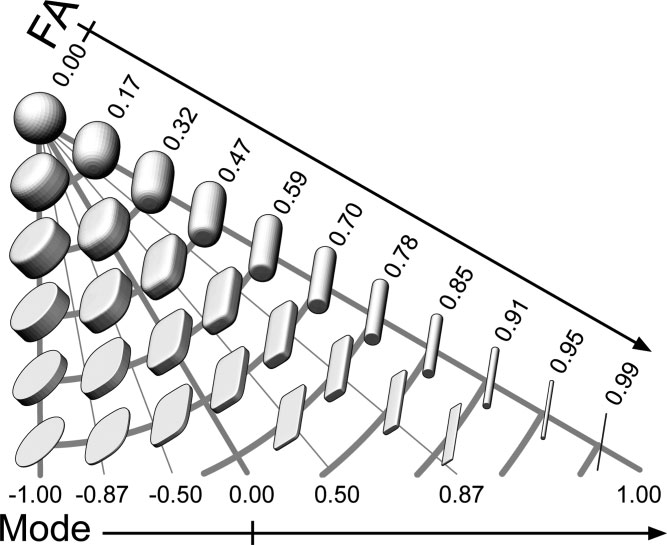
\includegraphics[width=0.5\textwidth]{pictures/-001.png}
	\caption{Darstellung der fraktionalen Anisotropie und des Modus von Matrizen in Form von Superquadrics\cite{kindlmann2004superquadric}. Die Fraktionale Anisotropie nimmt mit gr\"o{\ss}erer Entfernung zum obersten linken Superquadric zu. Der Modus des Deviators wird abh\"angig vom Winkel dargestellt, wobei er links -1 betr"agt und rechts 1. Entnommen aus \cite[S.~140]{ennis2006orthogonal}.}
	\label{Modus}
\end{figure}
Um die Intuition hinter dem Modus zu verdeutlichen, sind in Abbildung \ref{Modus} Superquadrics von Matrizen unterschiedlicher Modi dargestellt. Insbesondere wird dadurch betont, dass der Modus nicht von der Gr\"o{\ss}e der Eigenwerte abh\"angt, sondern von deren Verteilung.

\subsubsection{Gradient}
Der Gradient einer skalaren Funktion $f: \mathbb{R}^n \rightarrow \mathbb{R}$  \"uber einem kartesischen Koordinatensystem ist definiert als

\begin{equation}
	grad(f) = 	
	\begin{pmatrix}
		\frac{\partial f}{\partial x_1} \\
		\vdots \\
		\frac{\partial f}{\partial x_n}
	\end{pmatrix}
\end{equation}

also als Vektor aller partiellen Ableitungen in die Richtungen $x_i$. Analog ist der Gradient einer Skalarfunktion $g: K^{m\times n} \rightarrow \mathbb{R}$, wobei $K^{m\times n}$ der Raum aller $m\times n$ Matrizen ist, definiert als

\begin{equation}
	grad(g) =
	\begin{pmatrix}
		\frac{\partial f}{\partial a_{11}} & \dots & \frac{\partial f}{\partial a_{1n}}  \\
		\vdots & \ddots & \vdots \\
		\frac{\partial f}{\partial a_{m1}} & \dots & \frac{\partial f}{\partial a_{mn}} 
	\end{pmatrix}
\end{equation}

wobei $a_{ij}$ die Komponenten der Matrizen sind.

\subsubsection{Orthogonalit\"at von Matrizen}
Zwei Matrizen $U,V$ werden als orthogonal zueinander bezeichnet, wenn \cite{ennis2006orthogonal}

\begin{equation}
tr(U,V^{T}) = 0
\end{equation}

\subsubsection{Matrixinvarianten}
\label{Matrixinvarianten}
Als Invarianten werden zu mathematischen Objekten zugeordnete Gr\"o{\ss}en bezeichnet, die invariant gegen\"uber der Anwendung bestimmten Transformationen auf die Objekte sind. Invarianten eines Tensors in Matrixdarstellung sind beispielsweise Gr\"o{\ss}en, die sich unab\"angig von der Wahl der Basis der Matrix nicht ver\"andern\cite{ennis2006orthogonal}. Eine Invariante ist somit eine Funktion $\Psi: M \rightarrow A$ die Objekten aus dem Vektorraum aller Matrizen $M$ Objekte aus der Menge $A$ zuordnet. In der Praxis wird f\"ur $A$ meistens $\mathbb{R}$ gew\"ahlt.

Da sich das vorliegende Paper auf symmetrische, dreidimensionale Tensoren 2. Grades und ausschlie{\ss}lich orthogonale Transformationen bezieht, werden die Invarianten eines Tensors $T$ durch seine Eigenwerte vollst\"andig charakterisiert. Invarianten sind in diesem Spezialfall also auch als Funktion $\Psi: \mathbb{R}^d \rightarrow \mathbb{R}$ der Form

\begin{equation}
	\Psi:
	\begin{bmatrix}
	\lambda_1\\
	\lambda_2\\
	\lambda_3
	\end{bmatrix}
	\rightarrow \mathbb{R}
\end{equation}

darstellbar, wobei $\lambda_1, \lambda_2, \lambda_3$ die Eigenwerte von $T$ sind. Die stimmt mit der Betrachtunsweise von Zobel und Scheuermann \cite{zobel2017extremal} \"uberein.

\subsubsection{Invariantens\"atze} 
Mengen von Invarianten werden als Invariantens\"atze bezeichnet.
Matrixinvarianten $\Psi_1$ und $\Psi_2$ werden als orthogonal zueinander bezeichnet, wenn ihre Gradienten f\"ur jede m\"ogliche Eingabematrix orthogonal sind. Die genauen Definitionen und Berechnungen dazu sind in `Orthogonal tensor invariants and the analysis of diffusion tensor magnetic resonance images' von Ennis, Kindlmann et al. \cite{ennis2006orthogonal} nachzulesen. Da Gradienten von skalarwertigen Funktionen auf Matrizen wiederum Matrizen sind \cite[S.~137]{ennis2006orthogonal}, gen\"ugt zu zeigen dass diese orthogonal zueinander sind. Invariantens\"atze, deren Elemente paarweise orthogonal sind, werden als orthogonale Invariantens\"atze bezeichnet.

F\"ur $3\times 3$ Matrizen enthalten alle orthogonalen Invariantens\"atze h\"oechstens 3 Invarianten. In der Praxis spielen jedoch eine Vielzahl von Invariantens\"atzen eine Rolle, von denen im Folgendenden einige erl\"autert werden:

\paragraph{Die Eigenwerte}

Eigenvektoren $v_i$, $1\leq i\leq 3$ einer 3 $\times$ 3 Matrix $M$ sind vom Nullvektor verschiedene Vektoren, f\"ur die gilt

\begin{equation}
	M \cdot v_i = \lambda_i v_i
\end{equation}

Intuitiv bedeutet das, dass sich durch Multiplikation mit $M$ ihre Richtung nicht ver\"andert. Die zugeh\"origen $\lambda_i$ werden als Eigenwerte bezeichnet und bilden einen orthogonalen Invariantensatz. Sie sind insbesondere in der Medizin sehr beliebt, da hohe Eigenwerte Hinweise auf Diffusionsbewegung in Gewebe liefern k\"onnen.

\paragraph{Der I-Invariantensatz}
Das charakteristische Polynom $\chi$ einer $3\times3$ Matrix $A$ hat die Form

\begin{equation}
	\centering
	\begin{split}
	&\chi_A(\lambda) = det(\lambda I - A)\\
	&\chi_A(\lambda) = -\lambda^3 + I_1\lambda^2 - I_2\lambda + I_3
	\end{split}
\end{equation}

wobei $\lambda$ ein Element aus dem K\"orper von $A$ und $I$ die dreidimensionale Einheitsmatrix ist. Es wird h\"aufig verwendet um die Eigenwerte von Matrizen zu bestimmen, da diese den Nullstellen entsprechen.

Eine weitere Eigenschaft ist, dass die Parameter $I_1, I_2, I_3$ einen Invariantensatz darstellen. Wegen der Wichtigkeit des charakteristischen Polynoms werden sie h\"aufig als `Hauptinvarianten' bezeichnet. Alternativ k\"onnen sie auch berechnet werden als

\begin{itemize}
	\item $I_1(A) = tr(A)$ (Spur von $A$)
	\item $I_2(A) = \frac{1}{2}(tr(A)^2 - tr(A^2))$ (Summe der Hauptminoren von $A$)
	\item $I_3(A) = det(A)$ (Determinante von $A$)
\end{itemize}
I bildet jedoch keinen orthogonalen Invariantensatz.

\paragraph{Der J-Invariantensatz}
Die Berechnung der J-Invarianten ist identisch zum I-Invariantensatz, nur dass statt $A$ der Deviator von $A$ als Eingabe verwendet wird:

\begin{itemize}
	\item $J_1(A) = tr(\tilde{A})$ (Spur des Deviators von $A$)
	\item $I_2(A) = \frac{1}{2}(tr(\tilde{A})^2 - tr(\tilde{A}^2))$ (Summe der Hauptminoren des Deviators von $A$)
\item $I_3(A) = det(\tilde{A})$ (Determinante des Deviators von $A$)
\end{itemize}

Dabei ist jedoch zu beachten, dass

\begin{equation}
	\begin{split}
	tr(\tilde{A}) &= tr(A - \frac{1}{3}tr(A)I)\\
	&= a_{11} - \frac{1}{3} tr(A) + a_{22} - \frac{1}{3} tr(A) + a_{33} - \frac{1}{3} tr(A)\\
	&= a_{11} + a_{22} + a{33} - tr(A)\\
	&= tr(A) - tr(A)\\
	&= 0
	\end{split}
\end{equation}

weshalb statt $J_1$ in der Regel $I_1$ als Invariante verwendet wird. \"Ahnlich wie I ist auch J nicht orthogonal.

\paragraph{Der K-Invariantensatz}
Der K-Invariantensatz ist orthogonal und besteht aus den Invarianten $K_1, K_2$ und $K_3$. Diese sind f\"ur eine Matrix $A$ definiert als

\begin{itemize}
	\item $K_1(A)=tr(A)$ (Spur von $A$)
	\item $K_2(A)=norm(\tilde{A})$ (Norm des Deviators von A)
	\item $K_3(A)=mode(\tilde{A})$ (Modus des Deviators von A)
\end{itemize}


\begin{figure}
	\centering
	\label{cylinderCoords}
	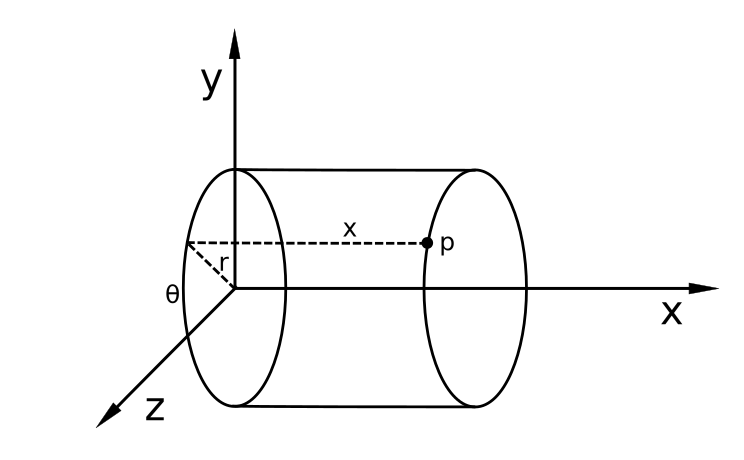
\includegraphics[width=0.5\textwidth]{pictures/cylinder}
	\caption{In dieser Abbildung werden zylindrische Koordinaten innerhalb eines kartesischen Koordinatensystems dargestellt. $x,y$ und $z$ entsprechen dabei den kartesischen Achsen. Die Koordinaten des Punktes $p$ sind angegeben als $x, r, \theta$. $x$ entspricht der kartesischen Koordinate, $r$ ist die Entfernung zwischen der Projektion von $p$ auf die von $y$ und $z$ Achse aufgespannte Fl\"ache und dem Koordinatenursprung und $\theta$ entspricht dem Winkel zwischen Projektion von $p$, dem Koordinatenursprung und der $x$-Achse. }
\end{figure}

Da $K_1 \in [-\infty, \infty]$, $K_2 \in [0,\infty]$, $K_3 \in [-1,1]$ bietet sich f\"r den K-Invariantensatz eine Darstellung in einem zylindrischen Koordinatensystem an, wobei $K_1$ eine Position auf einer zentralen Achse beschreibt, $K_2$ die orthogonale Entfernung zu diesem Punkt und $K_3$ den Winkel zu einer festgelegten, zur zentralen Achse orthogonalen, zweiten Achse. Sowohl ein zylindrisches als auch ein kartesisches Koordinatensystem sind in Abbildung \ref{cylinderCoords} dargestellt. $K_1$ entspricht dabei der zylindrischen $x$-Koordinate, $K_2$ dem Radius $r$ und $K_3$ dem Winkel $\theta$



\paragraph{Der R-Invariantensatz}
Der orthogonale R-Invariantensatz verwendet die Invarianten $R_1, R_2$ und $R_3$. F\"ur eine Matrix $A$ sind sie definiert als

\begin{itemize}
	\item $R_1(A)=norm(A)$ (Norm von $A$)
	\item $R_2(A)=\sqrt{\frac{3}{2}} \frac{norm(\tilde{A})}{norm(A)}$ (Fraktionale Anisotropie)
	\item $R_3(A)=mode(A)$ (Modus von $A$)
\end{itemize}

Dabei f\"allt auf, dass $R_3(A) = K_3(A) = mode(A)$. \"Ahnlich wie der K-Invariantensatz kann auch R in einem zylindrischen Koordinatensystem dargestellt werden.

\begin{figure}
	\centering
	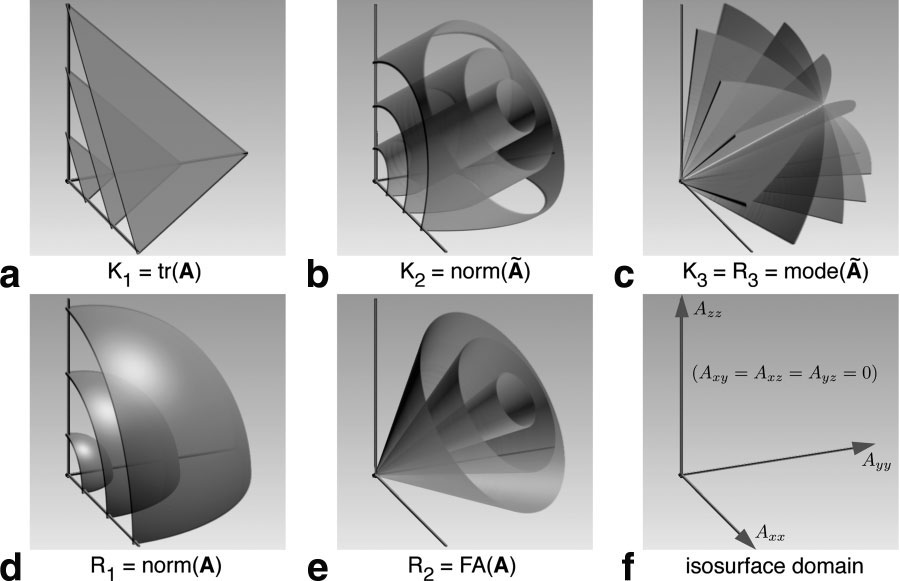
\includegraphics[width=0.5\textwidth]{pictures/-000.png}
	\caption{Dargestellt sind Isofl\"achen der K und R Invarianten von diagonalisierten $3\times 3$ Matrizen (alle Werte ausserhalb der Hauptdiagonale sind 0). Die Koordinatenachsen entsprechen den drei Eigenwerten der Matrizen. Entnommen aus \cite[S.~139]{ennis2006orthogonal}}
	\label{KRInvariants}
\end{figure}

Sowohl K als auch R beschreiben die Verteilung, die Gr\"o{\ss}e und das Verh\"altnis der Eigenwerte zueinander. Dies ist in Abbildung \ref{KRInvariants} dargestellt. 

\subsection{Mechanische Grundlagen}
\subsubsection{Physikalisches Feld}
Ein physikalisches Feld ist eine physikalische Gr\"o{\ss}e, die an verschiedenen Positionen im Raum unterschiedliche Werte annimmt\cite[1–2 Electric and magnetic fields]{feynman2011feynman}. Abstrahiert kann es als Funktion $\mathbb{R}^n \rightarrow V$ beschrieben werden, wobei $V$ eine beliebige Menge ist. H\"aufig wird f\"ur $V$ jedoch $\mathbb{R}$ (z.B. bei Temperaturen), $\mathbb{R}^n$ (z.B. bei Str\"omungen) oder $\mathbb{R}^{m\times n}$ (z.B. bei Verformungen) eingesetzt. Andere Beispiele f\"ur physikalische Felder sind elektromagnetische Felder oder Gravitationsfelder. Felder werden meist abh\"angig von ihrem Bild klassifiziert, so z.B. in Skalar-, Vektor- oder Tensorfelder.

Wenn Felder nicht in Form einer kontinuierlichen Funktion beschrieben werden k\"onnen, zum Beispiel weil nur f\"ur endlich viele Punkte Messwerte vorhanden sind, kann ein Feld auf einem Gitter, das aus diesen Messpunkten besteht, definiert werden. Die Werte innerhalb der Zellen lassen sich dann durch Interpolation der Werte an den Eckpunkten berechnen.


Innerhalb der vorliegenden Arbeit werden Spannung und Verformung an Punkten von Objekten als Felder $\mathbb{R} \rightarrow \mathbb{R}^{m\times n}$ beschrieben.


\subsubsection{Mechanische Spannung}
In der Mechanik beschreibt Spannung (engl. stress) die Kraft, die Partikel innerhalb eines Objektes aufeinander auswirken. Um die Spannung an einem Punkt zu bestimmen, wird die Kraft, die auf infinitesimal kleine Fl\"achenteile von Schnitten durch das Objekt wirkt, berechnet. Die Kraft ist dabei als Vektor formulierbar. Wenn die Schnitte entlang von 3 zueinander orthogonalen Ebenen durchgef\"uhrt werden, erh\"alt man so drei Vektoren, die zusammen die Matrixdarstellung des Cauchy Tensors $\sigma$ bilden:

\begin{equation}
	\sigma =  
	\begin{bmatrix}
		\sigma_x & \tau_{xy} & \tau_{xz}\\
		\tau_{xy} & \sigma_y & \tau_{yz}\\
		\tau_{xz} & \tau_{yz} & \sigma_z
	\end{bmatrix}
\end{equation}

Jede Spalte des Cauchy Tensors entspricht dabei einem der Vektoren. Wie aus der Formel ersichtlich, ist die Matrix symmetrisch und enth\"alt zwei Typen von Komponenten: Die $\sigma$ entlang der Hauptdiagonale, die Kraft in Richtung der Normalen der jeweiligen Ebene angeben, und den $\tau$, die Scherspannungen angeben, die parallel zu den Schnittebenen verlaufen. 

\subsubsection{Mechanische Verformung}
Wenn in einem Objekt Spannung vorliegt, so verformt es sich proportional zur St\"arke der Spannung (Hookesches Gesetz). Durch einen Verformungstensor (auch Verzerrungstensor, engl. strain tensor) l\"asst sich die Verformung an einem Punkt durch Kraftanwendung angeben:

\begin{equation}
	\epsilon =  
	\begin{bmatrix}
		\epsilon_x & \frac{1}{2}\gamma_{xy} & \frac{1}{2}\gamma_{xz}\\
		\frac{1}{2}\gamma_{xy} & \epsilon_y & \frac{1}{2}\gamma_{yz}\\
		\frac{1}{2}\gamma_{xz} & \frac{1}{2}\gamma_{yz} & \epsilon_z
	\end{bmatrix}
\end{equation}

\"Ahnlich wie beim Spannungstensor dr\"ucken die $\epsilon$ in der Hauptdiagonale Dehnungen oder Stauchungen des Objektes entlang der Hauptachsen aus, die $\gamma$ Werte Scherungen, also Verschiebungen der Seitenfl\"achen zueinander. Dabei \"andern sich die Winkel der Kanten des Objektes zueinander.

\section{Verwendete Verfahren und Technologien}
\label{sec:Technologien}
\subsection{FAnToM}
FAnToM\cite{fantomWebsite}\cite{wiebel2009fantom} (`Field Analysis using Topological Methods') ist ein Programm, dessen Entwicklung im Jahre 1999 begann. Obwohl es zu Anfang noch als Hilfsmittel f\"ur die Analyse von Vektorfeldtopologien konzipiert war, entwickelte es sich \"uber die Jahre hinweg zu einer Plattform f\"ur diverse Visualisierungen.

Erweiterungen von FAnToM werden in Form von sogenannten Algorithmen entwickelt. Dabei unterscheidet man 2 Arten: den `Data Algorithm' und den `Visualization Algorithm'. Data Algorithms sind Erweiterungen, die Daten verarbeiten. Beispiele daf\"ur sind `Load VTK', eine Erweiterung die Daten aus dem VTK Format einliest, oder `Combine Scalar to Vector', das mehrere Felder mit skalaren Werten zu einem einzelnen Feld mit Vektorwerten kombiniert, deren Komponenten den Skalaren entsprechen.
Visualization Algorithms dagegen dienen dazu, Visualisierungen zu erzeugen. Interaktionen mit der den Visualisierungen k\"onnen entweder \"uber die Maus oder \"uber Optionen stattfinden.

Ein wesentliches Feature von FAnToM besteht darin, Algorithmen miteinander zu verkn\"upfen. Dies geschieht, indem Ausgabedaten von Algorithmen k\"onnen als Eingabe f\"ur andere dienen k\"onnen. Da viele Algorithmen mit Blick auf Wiederverwendbarkeit entwickelt wurden, k\"onnen so mit wenig Aufwand aus bestehenden Algorithmen komplett neue Visualisierungspipelines entwickelt werden.

Erweiterungen k\"onnen auf eine Vielzahl von m\"achtigen Werkzeugen zugreifen, die von FAnToM zur Verf\"ugung gestellt werden. Besonders wichtig f\"ur die vorliegende Arbeit waren dabei das hoch entwickelte (ToDo: anderes Wort) Datenmodell, das viele Funktionen zum Verarbeiten von Feldern und Tensoren bietet, die bestehenden Schnittstellen f\"ur Qt und OpenGL sowie die gro{\ss}e Bibliothek von wiederverwendbaren Algorithmen.
\subsection{OpenGL}
OpenGL\cite{openglWebsite} ist eine Spezifikation die das Verhalten eines rasterbasierten Renderingsystems beschreibt. Sie definiert eine Schnittstelle, gegen die von zwei Seiten entwickelt werden kann: Zum einen von Seiten der Hardwarehersteller, die Funktionen von OpenGL auf ihrer Hardware implementieren. Zum anderen von Programmierern, die durch OpenGL unabh\"angig von der Hardware, auf der das Programm am Ende laufen soll, entwickeln k\"onnen. 

Die Verarbeitungsschritte von der \"Ubergabe von Daten zu OpenGL bis zum fertig gerenderten Bild wird als Rendepipeline bezeichnet. Seit Version 2.0 unterst\"utzt OpenGL sogenannte `Shader', kleine Programmst\"ucke, die es Benutzern von OpenGL erm\"oglicht, die Renderpipeline sehr stark zu ver\"andern. Shader bekommen drei Arten von Eingabedaten:

\begin{enumerate}
	\item Die Ausgabe des vorherigen Schrittes in der Renderpipeline
	\item Parameter aus dem Programm, das OpenGL verwendet (`Uniforms')
	\item Daten, die aus dem vorhergehenden Shader \"ubergeben wurden
\end{enumerate}

Ein wichtiger Spezialfall von Uniforms sind Texturen, die in dem OpenGL verwendenden Programm geladen, an die Shader \"ubergeben und dort verwendet werden k\"onnen.

In der vorliegenden Arbeit wurden Vertex, Geometry und Fragment Shader entwickelt. Diese drei Typen sind folgend kurz erkl\"art.

\paragraph{Vertex Shader}
Vertex Shader bekommen als Eingabe aus der Renderpipeline die Punkte eines zu zeichnenden Grafikprimitivs, beispielsweise Punkte eines Liniensegmentes oder die Eckpunkte eines Dreiecks. Abh\"angig von den eingegebenen Uniforms k\"onnen die Koordinaten dieser Punkte dann durch den Shader ver\"andert werden. Dies ist beispielsweise \"ublich um die Sicht auf die Szene von der Position der Kamera aus zu berechnen. Vertex Shader werden einmal pro Punkt ausgef\"uhrt. Die Ausgabe des Vertex Shaders sind die neuen Koordinaten der Punkte der Primitive.

\paragraph{Geometry Shader}
Die Renderpipeline \"ubergibt dem Geometry Shader f\"ur jedes Primitiv eine Liste der dazugeh\"orenden Punkte, zum Beispiel eine Liste von 3 Punkten f\"ur ein Dreieck. Der Geometry Shader ist in der Lage, die Position und den Typ dieser Primitive beliebig zu ver\"andern, und sogar neue Punkte zu erzeugen. So kann er bespielsweise aus einer Linie ein Dreieck erzeugen. Zus\"atzlich kann er pro Punkt Uniforms definieren, die an sp\"ater ausgef\"uhrte Shader (Vertex Shader) weitergegeben werden. Pro Primitv wird der Geometry Shader einmal ausgef\"uhrt.

\paragraph{Fragment Shader}
Fragment Shader bestimmen die Farben der Fragmente. Fragmente sind St\"ucke der projizierten Primitve, deren Gr\"o{\ss}e von der Art der Rasterisierung abh\"angen (z.B. Supersampling). Die Eingaben sind der Mittelpunkt des Fragments und die f\"ur diesen Punkt interpolierten Attribute der Eckpunkte des Primitivs. Neben der Fragmentfarbe k\"onnen auch Werte ausgegeben werden, zum Beispiel ein Tiefenattribut, das korrekte \"Uberlappung von Primitiven erm\"oglicht.

Weitere im Folgenden verwendete Funktionen von OpenGL sind `Blending', eine Funktion durch die Fragmente \"ubereinander gezeichnet und ihre Farbwerte gewichtet kombininert werden k\"onnen, was z.B. f\"ur transparente Objekte wichtig ist sowie die M\"oglichkeit, gerenderte Bilder in einer Textur zu speichern.

Die meisten Implementierungen von OpenGL machen intensiven Gebrauch von Grafikkarten und deren F\"ahigkeit zur extremen Parallelisierung von Aufgaben. Dies, verbunden mit der M\"oglichkeit Ausgaben der Renderpipeline zur\"uck in den Arbeitsspeicher zu laden und der Anpassbarkeit der Renderpipeline durch Shader erm\"oglicht es, OpenGL auch f\"ur andere rechenintensive, jedoch gut parallelisierbare Aufgaben zu benutzen und so Berechnungen stark zu beschleunigen.

\subsection{Direct Volume Rendering}
In der Computergrafik werden dreidimensionale Objekte \"ublicherweise durch Dreiecke dargestellt, durch die die Oberfl\"ache der Objekte approximiert werden. Dies entfernt jedoch alle Informationen \"uber Strukturen im Inneren der Objekte, so wie Bereiche unterschiedlicher Materialien oder Dichte. Durch das Berechnen und Zeichnen von Isofl\"achen kann dieses Problem behoben werden, dies erfordert jedoch hohe Rechenzeiten und gute Kenntnis der Datens\"atze, um geeignete Isowerte festzulegen.


\begin{figure}
	\begin{minipage}{0.5\textwidth}
		\centering
		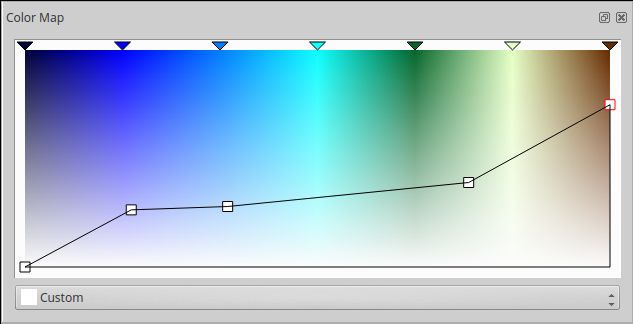
\includegraphics[width=0.9\textwidth]{pictures/Colormap.png}
		\caption{Eine Implementierung einer interaktiven Transferfunktion in FAnToM. }
		\label{Colormap}
	\end{minipage}
	\hspace{0.5cm}
	\begin{minipage}{0.5\textwidth}
		\centering
		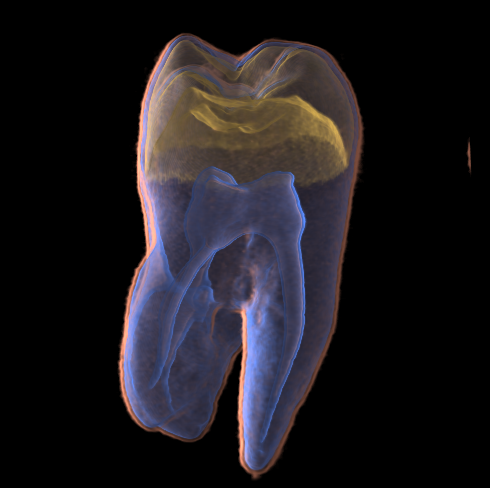
\includegraphics[width=0.47\textwidth]{pictures/Zahn.png}
		\caption{Ein Direct Volume Rendering eines Zahns. Entnommen aus \cite[S.~6]{drebin1988volume}}
		\label{Zahn}
	\end{minipage}
\end{figure}
Eine Alternative bietet das Direct Volume Rendering\cite{drebin1988volume} (im Folgenden DVR). Als Eingabe wird ein Feld $f: \mathbb{R}^3\rightarrow\mathbb{R}$ verwendet, das Punkten im dreidimensionalen Raum skalare Werte zuordnet. Die Interpretation dieser Werte kann, abh\"angig vom Einsatzgebiet, unterschiedlich sein. Beispiele daf\"ur sind die abgegebene Energie von Regionen in der Magnetresonanztomographie oder die Menge von absorbierter R\"ontgenstrahlung in der Computertomographie. Den skalaren Werte werden mittels einer `Transferfunktion' Farbwerte und Transparenz zugeordnet.

Eine Implementierung einer Interaktiven Transferfunktion in FAnToM ist in Abbildung \ref{Colormap} zu sehen. Die horizontale Achse entspricht den skalaren Werten zwischen Minimum und Maximum im Datensatz sowie den zugeordneten Farben. Die vertikale Achse entspricht der Transparenz, von vollst\"andig transparent am unteren Rand bis zu komplett intransparent am oberen Rand. Durch Position und Farbe der Dreiecke am oberen Rand der Transferfunktion kann die Farbzuordnung festgelegt werden. Die Quadrate stellen interaktiv ausgew\"ahlte Punkte dar, die Zuordnungen von Werten im Skalarfeld zu Farb- und Transparenzwerten entsprechen, zwischen denen entlang der verbindenden Linien interpoliert wird. So werden allen Werten im Feld eine Farbe und eine Transparenz zugeordnet. 

Ziel des DVR ist es, mithilfe der Transferfunktion eine dreidimensionale Darstellung des Feldes zu erzeugen, in der Bereiche entsprechend der Transferfunktion Licht ausstrahlen, das von anderen Bereichen entsprechend ihrer Transparenz durchgelassen oder absorbiert wird. Dadurch ist es m\"oglich, Strukturen im Inneren des Feldes sichtbar zu machen. Ein Beispiel f\"ur eine so erzeugtes Bild ist in Abbildung \ref{Zahn} dargestellt.

Es existieren viele DVR Verfahren die sich in Laufzeit, Bildqualit\"at und Anf\"alligkeit f\"ur Artefakte unterscheiden. In dieser Arbeit wurde Raycasting verwendet, was folgend erl\"autert wird.

\subsubsection{Raycasting}
\begin{figure}
	\centering
	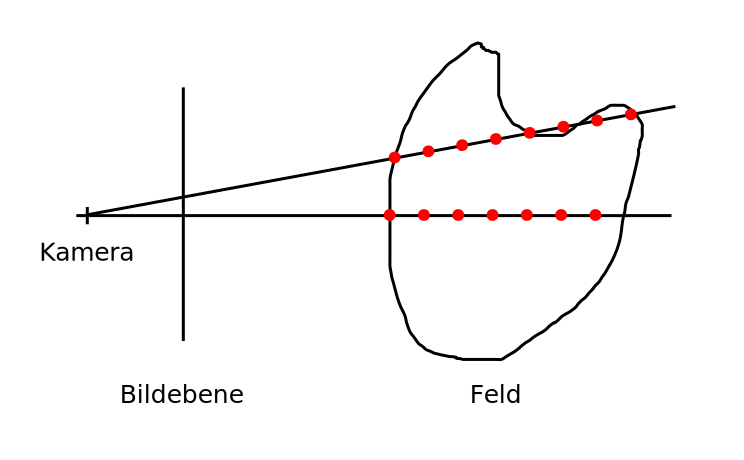
\includegraphics[width=0.5\textwidth]{pictures/Raycasting}
	\caption{Eine vereinfachte Darstellung eines optimierten Raycastings. Die Bildebene entspricht der Ebene, die durch die durch die imagin\"are Position der Pixel gebildet wird. Die Roten Punkte entlang der Strahlen entsprechen den Samplepunkten.}
	\label{Raycasting}
\end{figure}
Beim Raycasting wird f\"ur jedes Pixel ein Strahl durch den Mittelpunkt des Pixels und die Position der Kamera berechnet. Entlang dieses Strahls wird an, nach ihrer Entfernung von der Kamera geordneten Punkten  $s_1, \dots, s_n$ (`Samplepunkten') der interpolierte Wert des Feldes $v(s_i), 1\leq i\leq n$ berechnet. Der paarweise Abstand der Samplepunkte ist dabei kontant. Aus dem ermittelten Wert wird mithilfe der Transferfunktion die Farbe $f(v(s_i))$ und die Transparenz $t(v(s_i))$ f\"ur diesen Wert bestimmt.

Dabei sei die Transparenz ein Wert im Intervall $[0,1]$ und Farbe ein Vektorraum \"uber $\mathbb{R}$, wie zum Beispiel im RGBA Farbmodell, f\"ur den die Multiplikation mit einem Skalar definiert ist. Die Farbe des Pixels $p$ wird dann f\"ur die Samplepunkte entlang des entsprechenden Strahls berechnet als

\begin{equation}
	p = \sum_{i=1}^{n} \left(f(s_i) \cdot \prod_{j=1}^{i} \frac{(1-t(s_j))}{n}\right)
	\label{RaycastingFormula}
\end{equation}

Das hat den Effekt, dass weiter von der Kamera entfernte Samplepunkte von n\"aheren Punkten entsprechend ihrer Transparenz verdeckt werden. Insbesondere hat es die Konsequenz, dass, sobald gen\"ugend Punkte verarbeitet wurden, so dass die `verbleibende Transparenz' einen Grenzwert unterschreitet, sich die Farbe des Pixels nicht mehr stark ver\"andert, und die Berechnung fr\"uhzeitig beendet werden kann. Die verbleibende Transparenz wird durch die Gesamtzahl der Samplepunkte $n$ geteilt, damit eine h\"ohere Anzahl an Samplepunkten nicht zu einem schnelleren Verlust von Transparenz f\"uhrt.

Eine weitere Optimierung besteht darin, die Samplepunkte erst nach dem Eintreten des Strahls in das Feld beginnen zu lassen und die Berechnung zu beenden, sobald alle verbleibenden Samplepunkte ausserhalb des Feldes liegen. Eine vereinfachte Darstellung dieses optimierten Verfahrens ist in \ref{Raycasting} dargestellt.
 
\begin{figure}
	\begin{subfigure}{0.30\textwidth}
		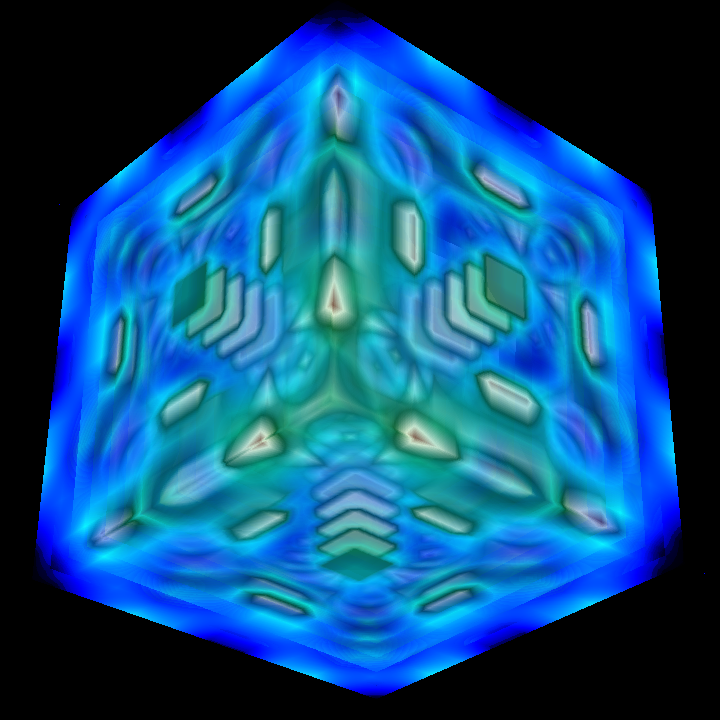
\includegraphics[width=\textwidth]{pictures/DVR1.png}
		\subcaption{}
		\label{SamplingPoints1}
	\end{subfigure}
	\hfill
	\begin{subfigure}{0.30\textwidth}
		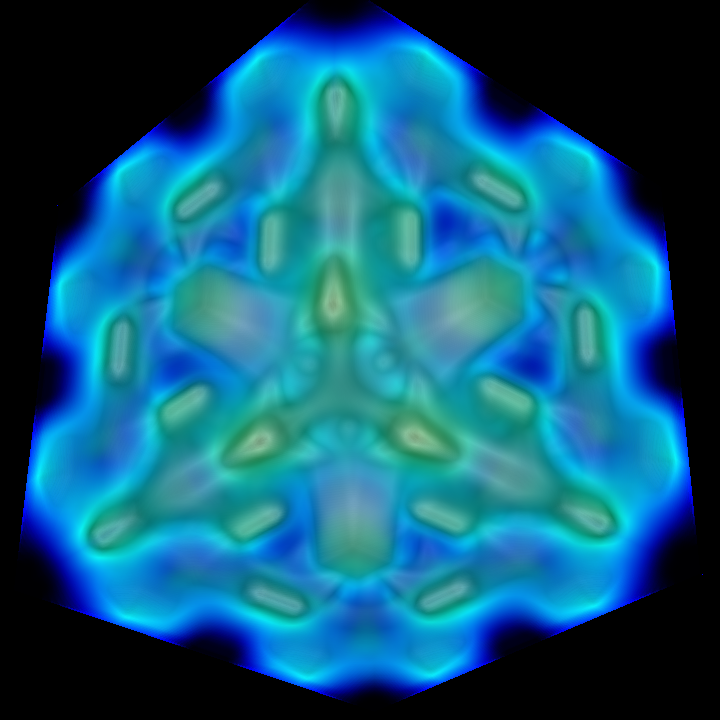
\includegraphics[width=\textwidth]{pictures/DVR2.png}
		\subcaption{}
		\label{SamplingPoints2}
	\end{subfigure}
	\hfill
	\begin{subfigure}{0.30\textwidth}
		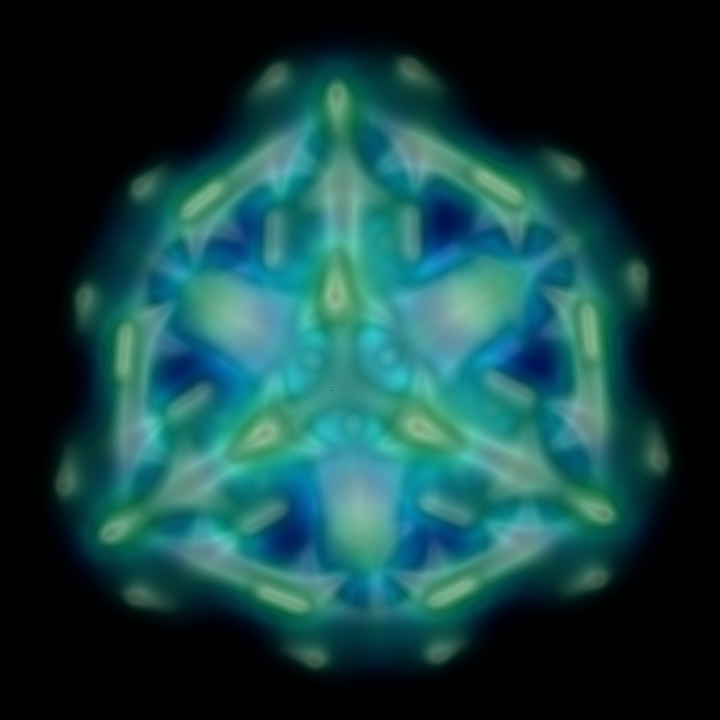
\includegraphics[width=\textwidth]{pictures/DVR3.png}
		\subcaption{}
		\label{SamplingPoints3}
	\end{subfigure}
	\caption{Drei Raycastings des Felds $f:\mathbb{R}^3\rightarrow\mathbb{R}, f\left(\protect\begin{array}{c}x\\y\\z\protect\end{array}\right)=cos(x\cdot y\cdot z)$.}
	\label{SamplingPoints}
\end{figure}

Die Qualit\"at eines Raycastings ist stark abh\"angig von der Anzahl an Samplepunkten pro Strahl und somit vom Abstand zwischen den Samplepunkten. Ein geringerer Abstand f\"uhrt generell zu weniger Artefakten und macht kleine Strukturen besser erkennbar, erh\"oht jedoch den Rechenaufwand. Indem der Benutzer die Anzahl von Samplepunkten selbst ausw\"ahlt, kann er seinen optimalen Tradeoff zwischen Rechenzeit und Bildqualit\"at finden. In Abbildung \ref{SamplingPoints1} und \ref{SamplingPoints2} sind zwei Darstellungen desselben Skalarfeldes zu sehen, die durch Raytracing mit einer unterschiedlichen Anzahl von Samplepunkten erzeugt wurden. \ref{SamplingPoints1} wurde mit 20 Samplepunkten erstellt, wodurch visuelle, scheibenartige Artefakte entstanden. Bei einer h\"oheren Menge von 200 Samplepunkten in \ref{SamplingPoints2} verschwinden diese Artefakte.

Eine weitere wichtige Einstellung ist, welche Zahl in Formel \ref{RaycastingFormula} f\"ur Variable $n$ verwendet wird. Wenn $n$ die Anzahl der Samplepunkte pro Strahl ist, kann dies, wenn die Blickrichtung der Kamera nicht senkrecht auf einer der Seitenfl\"achen steht, dazu f\"uhren, dass Bereiche am Rand des Feldes transparenter dargestellt werden als in der Mitte. Das liegt daran, dass der Strahl am Rand weniger Samplepunkte produziert die innerhalb des Feldes liegen. Ein Beispiel daf\"ur ist in \ref{SamplingPoints3} mit 200 Samplepunkten dargestellt. 

Alternativ kann f\"ur $n$ die Anzahl der Samplepunkte, die tats\"achlich im Feld liegen, gew\"ahlt werden. Dies wurde in Abbildung \ref{SamplingPoints2} getan. Wenn man nun \ref{SamplingPoints2} und \ref{SamplingPoints3} miteinander vergleicht, f\"allt auf, dass die Pixel in der mitte der Darstellung etwa die gleichen Farben erhalten haben, \ref{SamplingPoints3} in Richtung Rand jedoch erheblich transparenter wird. Welche von beiden Varianten bevorzugt wird, h\"angt von der Art des Datensatzes ab sowie davon, wie wichtig es ist, korrekte Werte ablesen und vergleichen zu k\"onnen.

\subsection{Contiuous Scatterplotting}
\subsubsection{Scatterplotting}
\begin{figure}
	\hspace{2cm}
	\begin{subfigure}{0.30\textwidth}
		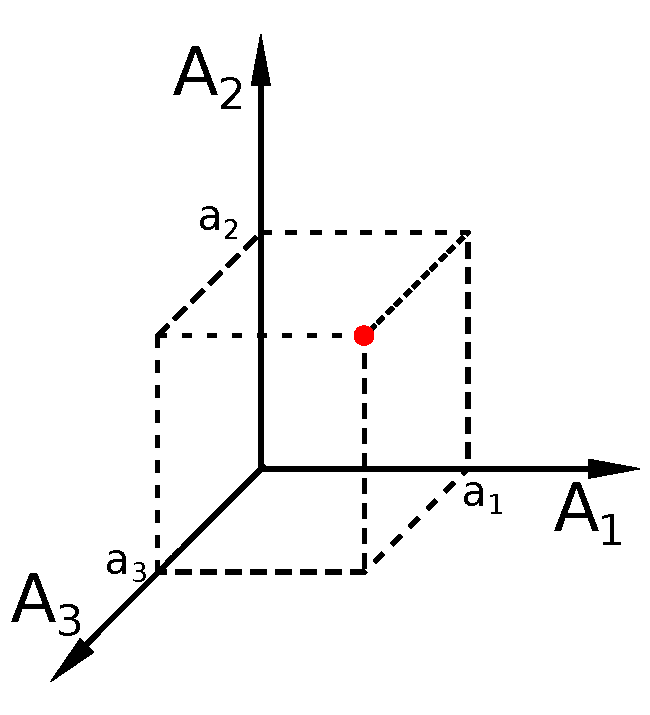
\includegraphics[width=\textwidth]{pictures/Scatterplot3D}
		\caption{}
	\end{subfigure}
	\hfill
	\begin{subfigure}{0.30\textwidth}
		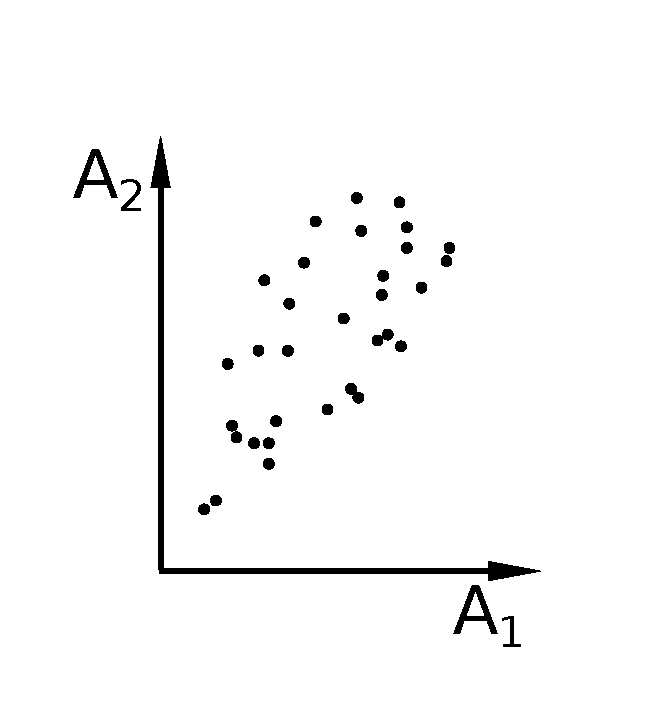
\includegraphics[width=\textwidth]{pictures/Scatterplot2D}
		\caption{}
	\end{subfigure}
	\hspace{2cm}
	\caption{Zwei Beispiele f\"ur Scatterplottings. In (a) wird ein Objekt mit den Attributwerten $a_1, a_2, a_3$ als roter Punkt in einem dreidimensionalen Scatterplot dargestellt. Um die Attribute besser ablesen zu k\"onnen, wurden gestrichelte Linien eingezeichnet. In (b) wurden mehrere Objekte mit unterschiedlichen Attributen im selben, zweidimensionalen Scatterplot als schwarze Punkte eingezeichnet.}
	\label{Scatterplots}
\end{figure}

Scatterplotting ist ein weiter verbreitetes Verfahren, um Attribute von Objekten relativ zueinander darzustellen. Es bildet eine Funktion auf einer Menge von Objekten $M$ als $\tau: M \rightarrow \mathbb{R}^n,n\in\{1,2,3\}$, wobei das Bild eine Projektion auf einzelne oder zusammengesetzte Attribute der Objekte darstellt.  Dazu wird pro Objekt ein Punkt in ein in zwei- oder dreidimensionales Koordinatensystem eingetragen, dessen Koordinatenachsen Attributwerten entsprechen. Beispiele f\"ur Scatterplottings sind in Abbildung \ref{Scatterplots} abgebildet. Das Bild von $\tau$ ist auf maximal 3 Dimensionen beschr\"ankt, da h\"oherdimensionale Daten visuell nur schwer zu interpretieren sind.

Ein Vorteil von Scatterplottings ist die leichte Erkennbarkeit von Strukturen in den Datens\"atzen: Cluster, Outlier und funktionale Zusammenh\"ange zwischen den verwendeten Attributen sind leicht erkennbar. 

Scatterplotting hat jedoch zwei gravierende Nachteile. Zum einen macht die geringe Dimensionalit\"at des Bildes von $\tau$ die Projektion auf eine Teilmenge der Attribute notwendig, zum anderen kann Scatterplotting nur endlich viele Objekte gleichzeitig darstellen. 

Ein Beispiel f\"ur ein Urbild mit unendlich vielen Elementen ist $\mathbb{R}^n$ bei physikalischen Feldern. Dort sind an jedem der unendlich vielen Punkte Werte definiert. Ein Scatterplot dieser unendlich vielen Elemente ist nun weder in endlicher Laufzeit m\"oglich, noch w\"aren einzelne Punkte in der entstehenden Darstellung erkennbar. Eine Alternative besteht darin, nur den Scatterplot der Eckpunkte der Zellen zu erzeugen, doch damit gehen Informationen \"uber die Punkte innerhalb der Zellen verloren.


\subsubsection{Erl\"auterung des Continuous Scatterplottings}
\begin{figure}
	\centering
	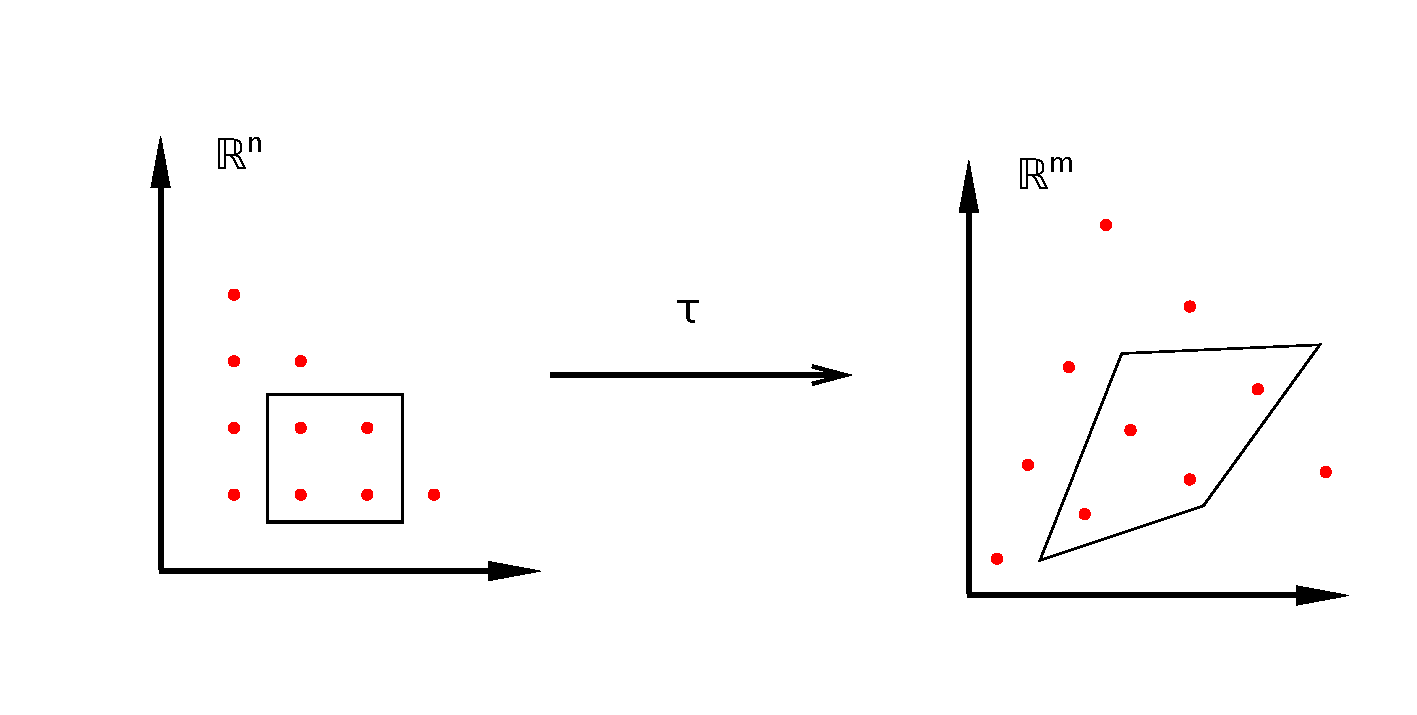
\includegraphics[width=0.5\textwidth]{pictures/ContinuousScatterplot}
	\caption{Darstellung der Dichteverteilung im Urbild und Bild von $\tau$. Die roten Punkte deuten die Dichte in den beiden Scatterplots an, die zwei Vierecke sind ein Bereich des Urbilds, der durch $\tau$ verformt wird. Zu erkennen ist, dass eine Streckung eines Bereichs zur Verringerung der Dichte und eine Stauchung zur Erh\"ohung der Dichte f\"uhrt. }
	\label{ContinuousScatterplot}
\end{figure}
Das Continuous Scatterplotting\cite{bachthaler2008continuous} stellt eine Erweiterung des Scatterplottings dar, so dass statt nur einer endlichen Anzahl von Objekten auch kontinuierliche Bereiche verarbeitet werden k\"onnen. Dabei verwendet es einen Ansatz, der dem Verfahren bei der Herleitung der Kontinuumsmechanik aus Systemem mit diskreten Massepunkten \"ahnelt \cite[S.~1429]{bachthaler2008continuous}. Das Ziel des Continuous Scatterplottings ist es eine Dichtefunktion $\sigma: \mathbb{R}^m \rightarrow \mathbb{R}$ zu finden, die den Punkten des Bildraums, abh\"angig von $\tau$, Dichtewerte zuordnet. In Abbildung \ref{ContinuousScatterplot} ist der Effekt, den $\tau$ auf die Dichtefunktion hat, dargestellt. Um $\sigma$ berechnen zu k\"onnen, werden 2 Annahmen getroffen:

Die erste Annahme ist, dass eine Dichtefunktion $s: \mathbb{R}^n \rightarrow \mathbb{R}$ existiert, die jedem Punkt des Urbilds von $\tau$ einen skalaren Wert, die Dichte an diesem Punkt, zuordnet. Der Einfachheit halber wird h\"aufig eine uniforme Dichte im gesamten Urbild angenommen. Aus der Dichte an den Punkten l\"asst sich die Gesamtdichte $M$, auch bezeichnet als Masse, einer Teilmenge $V\subset\mathbb{R}^n$ berechnen:

\begin{equation}
	M = \int_{V}s(x)d^nx
	\label{Dichtefunktion}
\end{equation}

Die zweite Annahme sagt aus, dass die Masse einer Teilmenge $V\subset\mathbb{R}^n$ gleich der Masse ihres Bildes ist, also $\tau$ die Gesamtdichte eines Bereichs nicht beeinflusst. F\"ur $\xi \in \mathbb{R}^m$ f\"uhren diese beiden Aussagen zu der Gleichung

\begin{equation}
M = \int_{V}s(x)d^nx = \int_{\phi = \tau(V)}\sigma(\xi)d^m\xi
\end{equation}

wodurch $\sigma$ eindeutig definiert ist.








\section{Umsetzung}
\label{sec:Umsetzung}
\subsection{Datenaufbereitung}
\subsection{Die Rasterisierung}
\subsection{Funktionen}
\subsection{Handbuch}
\subsection{Muss noch \"uberarbeitet werden}
\section{Ergebnisse}
\label{Ergebnisse}
\subsection{title}
\section{Ausblick}
\label{sec:Ausblick}
Fehler reduzieren durch Berechnung der Gr\"o{\ss}e des tats\"achlich belegten Volumens pro Tetraeder und Voxel -> Supersampling???
% %%%%%%%%%%%%%%%%%%%%%%%%%%%%%%%%%%%%%%%%%%%%%%%%%%%%%%%%%%%%%%
% HERE ENDS YOUR DOCUMENT
% %%%%%%%%%%%%%%%%%%%%%%%%%%%%%%%%%%%%%%%%%%%%%%%%%%%%%%%%%%%%%%

% Settings for the references (which are numbered in roman style)
\label{LastPageBeforeRefs}
\clearpage
\ofoot{\vspace{-0.1cm}\textbf{\large\thepage}/\textbf{\large\getpagerefnumber{LastBibPage}}}
\pagenumbering{Roman}

\defbibfilter{papers}{
	type=article or
	type=inproceedings
}
\printbibliography[type=book,title={Bücher}]
\printbibliography[filter=papers,title={Artikel}]
\printbibliography[type=online,title={Internetressourcen}]
\label{LastBibPage}
\end{document}
